\documentclass[conference]{IEEEtran}
\usepackage[utf8]{inputenc}   % <<<<< Linux
\usepackage[english]{babel} % <<<<< English
\newcommand{\acknowledgments}{@undefined} % new LaTeX variable name
\addto\captionsenglish{\renewcommand{\acknowledgments}{Acknowledgments}}
%\addto\captionsenglish{\renewcommand{\contentsname}{Contents}}
\addto\captionsenglish{\renewcommand{\listtablename}{List of Tables}}
\addto\captionsenglish{\renewcommand{\listfigurename}{List of Figures}}
%\addto\captionsenglish{\renewcommand{\nomname}{Nomenclature}}
%\addto\captionsenglish{\renewcommand{\bibname}{References}} % Bibliography
%\addto\captionsenglish{\renewcommand{\appendixname}{Appendix}}

% > Portuguese
%
\addto\captionsportuguese{\renewcommand{\acknowledgments}{Agradecimentos}}
%\addto\captionsportuguese{\renewcommand{\contentsname}{Conte\'{u}do}}
%\addto\captionsportuguese{\renewcommand{\listtablename}{Lista de Figuras}}
%\addto\captionsportuguese{\renewcommand{\listfigurename}{Lista de Tabelas}}
%\addto\captionsportuguese{\renewcommand{\nomname}{Lista de S\'{i}mbolos}} % Nomenclatura
%\addto\captionsportuguese{\renewcommand{\bibname}{Refer\^{e}ncias}} % Bibliografia
%\addto\captionsportuguese{\renewcommand{\appendixname}{Anexo}} % Apendice


\usepackage{graphicx}


% 'color' package
%
% Colour control for LaTeX documents.
% http://www.ctan.org/tex-archive/macros/latex/required/graphics/
%
% > defines color macros: \color{<color name>}
%
%\usepackage{color}


% 'amsmath' package
%
% Mathematical enhancements for LaTeX.
% http://www.ctan.org/tex-archive/macros/latex/required/amslatex/
%
% > American Mathematical Society plain Tex macros
%
%\usepackage{amsmath}  % AMS mathematical facilities for LaTeX.
\usepackage{mathtools}
\usepackage{amsthm}   % Typesetting theorems (AMS style).
\usepackage{amsfonts} % 


% 'wrapfig' package
%
% Produces figures which text can flow around.
% http://www.ctan.org/tex-archive/macros/latex/contrib/wrapfig/
%
% > wrap figures/tables in text (i.e., Di Vinci style)
%
% \usepackage{wrapfig}


% 'subfigure' package
%
% Deprecated: figures divided into subfigures.
% http://www.ctan.org/tex-archive/obsolete/macros/latex/contrib/subfigure/
%
% > subcaptions for subfigures
%
\usepackage{subfigure}


% 'subfigmat' package
%
% Automates layout when using the subfigure package.
% http://www.ctan.org/tex-archive/macros/latex/contrib/subfigmat/
%
% > matrices of similar subfigures
%
\usepackage{subfigmat}


% 'url' package
%
% Verbatim with URL-sensitive line breaks.
% http://www.ctan.org/tex-archive/macros/latex/contrib/url/
%
% > URLs in BibTex
%
% \usepackage{url}


% 'varioref' package
%
% Intelligent page references.
% http://www.ctan.org/tex-archive/macros/latex/required/tools/
%
% > smart page, figure, table and equation referencing
%
%\usepackage{varioref}


% 'dcolumn' package
%
% Align on the decimal point of numbers in tabular columns.
% http://www.ctan.org/tex-archive/macros/latex/required/tools/
%
% > decimal-aligned tabular math columns
%
\usepackage{dcolumn}
\newcolumntype{d}{D{.}{.}{-1}} % column aligned by the point separator '.'
\newcolumntype{e}{D{E}{E}{-1}} % column aligned by the exponent 'E'


% 'verbatim' package
%
% Reimplementation of and extensions to LaTeX verbatim.
% http://www.ctan.org/tex-archive/macros/latex/required/tools/
%
% > provides the verbatim environment (\begin{verbatim},\end{verbatim})
%   and a comment environment (\begin{comment},  \end{comment})
%
% \usepackage{verbatim}


% 'moreverb' package
%
% Extended verbatim.
% http://www.ctan.org/tex-archive/macros/latex/contrib/moreverb/
%
% > supports tab expansion and line numbering
%
% \usepackage{moreverb}



% 'nomencl' package
%
% Produce lists of symbols as in nomenclature.
% http://www.ctan.org/tex-archive/macros/latex/contrib/nomencl/
%
% The nomencl package makes use of the MakeIndex program
% in order to produce the nomenclature list.
%
% Nomenclature
% 1) On running the file through LATEX, the command \makenomenclature
%    in the preamble instructs it to create/open the nomenclature file
%    <jobname>.nlo corresponding to the LATEX file <jobname>.tex and
%    writes the information from the \nomenclature commands to this file.
% 2) The next step is to invoke MakeIndex in order to produce the
%    <jobname>.nls file. This can be achieved by making use of the
%    command: makeindex <jobname>.nlo -s nomencl.ist -o <jobname>.nls
% 3) The last step is to invoke LATEX on the <jobname>.tex file once
%    more. There, the \printnomenclature in the document will input the
%    <jobname>.nls file and process it according to the given options.
%
% http://www-h.eng.cam.ac.uk/help/tpl/textprocessing/nomencl.pdf
%
% Nomenclature (produces *.nlo *.nls files)
\usepackage{nomencl}
\makenomenclature
%
% Group variables according to their symbol type
%
\RequirePackage{ifthen} 
\ifthenelse{\equal{\languagename}{english}}%
    { % English
    \renewcommand{\nomgroup}[1]{%
      \ifthenelse{\equal{#1}{R}}{%
        \item[\textbf{Roman symbols}]}{%
        \ifthenelse{\equal{#1}{G}}{%
          \item[\textbf{Greek symbols}]}{%
          \ifthenelse{\equal{#1}{S}}{%
            \item[\textbf{Subscripts}]}{%
            \ifthenelse{\equal{#1}{T}}{%
              \item[\textbf{Superscripts}]}{}}}}}%
    }{% Portuguese
    \renewcommand{\nomgroup}[1]{%
      \ifthenelse{\equal{#1}{R}}{%
        \item[\textbf{Simbolos romanos}]}{%
        \ifthenelse{\equal{#1}{G}}{%
          \item[\textbf{Simbolos gregos}]}{%
          \ifthenelse{\equal{#1}{S}}{%
            \item[\textbf{Subscritos}]}{%
            \ifthenelse{\equal{#1}{T}}{%
              \item[\textbf{Sobrescritos}]}{}}}}}%
    }%


\usepackage{rotating}
\usepackage[pdftex]{hyperref} % enhance documents that are to be
                              % output as HTML and PDF
\hypersetup{colorlinks,       % color text of links and anchors,
                              % eliminates borders around links
%            linkcolor=red,    % color for normal internal links
            linkcolor=black,  % color for normal internal links
            anchorcolor=black,% color for anchor text
%            citecolor=green,  % color for bibliographical citations
            citecolor=black,  % color for bibliographical citations
%            filecolor=magenta,% color for URLs which open local files
            filecolor=black,  % color for URLs which open local files
%            menucolor=red,    % color for Acrobat menu items
            menucolor=black,  % color for Acrobat menu items
%            pagecolor=red,    % color for links to other pages
            pagecolor=black,  % color for links to other pages
%            urlcolor=cyan,    % color for linked URLs
            urlcolor=black,   % color for linked URLs
            bookmarks=true,         % create PDF bookmarks
            bookmarksopen=false,    % don't expand bookmarks
            bookmarksnumbered=true, % number bookmarks
            pdftitle={Thesis},
            pdfauthor={Andre C. Marta},
            pdfsubject={Thesis Title},
            pdfkeywords={Thesis Keywords},
            pdfstartview=FitV,
            pdfdisplaydoctitle=true}



\usepackage[figure,table]{hypcap}
\usepackage[
    backend=biber,
    style=ieee,
    sortlocale=en_EN,
    natbib=true,
    url=false,
    doi=true,
    eprint=false
]{biblatex}
\newrobustcmd*{\parentexttrack}[1]{%
  \begingroup
  \blx@blxinit
  \blx@setsfcodes
  \blx@bibopenparen#1\blx@bibcloseparen
  \endgroup}

\AtEveryCite{%
  \let\parentext=\parentexttrack%
  \let\bibopenparen=\bibopenbracket%
  \let\bibcloseparen=\bibclosebracket}

\makeatother
\addbibresource{extended_abstract.bib}

\usepackage{notoccite}

\usepackage{multirow}

\usepackage{booktabs}

\usepackage{pdfpages}

\usepackage{enumitem}
\usepackage{arydshln}
\usepackage{tikz}
\setlist{nosep}

\newcommand{\ud}{\mathrm{d}}                % total derivative
\newcommand{\degree}{\ensuremath{^\circ\,}} % degrees

\newcommand{\mcol}{\multicolumn}            % table format

\newcommand{\eqnref}[1]{(\ref{#1})}
\newcommand{\class}[1]{\texttt{#1}}
\newcommand{\package}[1]{\texttt{#1}}
\newcommand{\file}[1]{\texttt{#1}}
\newcommand{\BibTeX}{\textsc{Bib}\TeX}
\newcommand{\tr}[1]{{\ensuremath{\textrm{#1}}}}   % text roman
\newcommand{\tb}[1]{{\ensuremath{\textbf{#1}}}}   % text bold face
\newcommand{\ti}[1]{{\ensuremath{\textit{#1}}}}   % text italic
\newcommand{\mc}[1]{{\ensuremath{\mathcal{#1}}}}  % math calygraphy
\newcommand{\mco}[1]{{\ensuremath{\mathcalold{#1}}}}% math old calygraphy
\newcommand{\mr}[1]{{\ensuremath{\mathrm{#1}}}}   % math roman
\newcommand{\mb}[1]{{\ensuremath{\mathbf{#1}}}}   % math bold face
\newcommand{\bs}[1]{\ensuremath{\boldsymbol{#1}}} % math symbol
\def\bm#1{\mathchoice                             % math bold
  {\mbox{\boldmath$\displaystyle#1$}}%
  {\mbox{\boldmath$#1$}}%
  {\mbox{\boldmath$\scriptstyle#1$}}%
  {\mbox{\boldmath$\scriptscriptstyle#1$}}}
\newcommand{\boldcal}[1]{{\ensuremath{\boldsymbol{\mathcal{#1}}}}}% math bold calygraphy
\DeclareMathOperator*{\argmin}{\arg\!\min}
\DeclareMathOperator*{\argmax}{\arg\!\max}

\usepackage{tikz}
\usetikzlibrary{matrix,decorations.pathreplacing,calc}

\usepackage{bm}
%\usepackage[]{algorithm2e}

\usepackage{color}
\usepackage{listings}
\usepackage{caption}

\lstnewenvironment{algorithm}[1][] %defines the algorithm listing environment
{
    \refstepcounter{nalg} %increments algorithm number
    \captionsetup{labelformat=algocaption,labelsep=colon} %defines the caption setup for: it ises label format as the declared caption label above and makes label and caption text to be separated by a ':'
    \lstset{ %this is the stype
        mathescape=true,
        frame=single,
        captionpos=b,
        aboveskip=25pt,
        belowskip=25pt,
        numbers=none,
        keywordstyle=\color{black}\bfseries,
        keywords={for, input, output, return, datatype, function, in, if, else, foreach, while, begin, end, } %add the keywords you want, or load a language as Rubens explains in his comment above.
        xleftmargin=.04\textwidth,
        #1 % this is to add specific settings to an usage of this environment (for instnce, the caption and referable label)
    }
}
{}

\newcommand{\q}[1]{``#1''} 

% *** CITATION PACKAGES ***
%
%\usepackage{cite}
% cite.sty was written by Donald Arseneau
% V1.6 and later of IEEEtran pre-defines the format of the cite.sty package
% \cite{} output to follow that of the IEEE. Loading the cite package will
% result in citation numbers being automatically sorted and properly
% "compressed/ranged". e.g., [1], [9], [2], [7], [5], [6] without using
% cite.sty will become [1], [2], [5]--[7], [9] using cite.sty. cite.sty's
% \cite will automatically add leading space, if needed. Use cite.sty's
% noadjust option (cite.sty V3.8 and later) if you want to turn this off
% such as if a citation ever needs to be enclosed in parenthesis.
% cite.sty is already installed on most LaTeX systems. Be sure and use
% version 5.0 (2009-03-20) and later if using hyperref.sty.
% The latest version can be obtained at:
% http://www.ctan.org/pkg/cite
% The documentation is contained in the cite.sty file itself.






% *** GRAPHICS RELATED PACKAGES ***
%
\ifCLASSINFOpdf
  % \usepackage[pdftex]{graphicx}
  % declare the path(s) where your graphic files are
  % \graphicspath{{../pdf/}{../jpeg/}}
  % and their extensions so you won't have to specify these with
  % every instance of \includegraphics
  % \DeclareGraphicsExtensions{.pdf,.jpeg,.png}
\else
  % or other class option (dvipsone, dvipdf, if not using dvips). graphicx
  % will default to the driver specified in the system graphics.cfg if no
  % driver is specified.
  % \usepackage[dvips]{graphicx}
  % declare the path(s) where your graphic files are
  % \graphicspath{{../eps/}}
  % and their extensions so you won't have to specify these with
  % every instance of \includegraphics
  % \DeclareGraphicsExtensions{.eps}
\fi
% graphicx was written by David Carlisle and Sebastian Rahtz. It is
% required if you want graphics, photos, etc. graphicx.sty is already
% installed on most LaTeX systems. The latest version and documentation
% can be obtained at: 
% http://www.ctan.org/pkg/graphicx
% Another good source of documentation is "Using Imported Graphics in
% LaTeX2e" by Keith Reckdahl which can be found at:
% http://www.ctan.org/pkg/epslatex
%
% latex, and pdflatex in dvi mode, support graphics in encapsulated
% postscript (.eps) format. pdflatex in pdf mode supports graphics
% in .pdf, .jpeg, .png and .mps (metapost) formats. Users should ensure
% that all non-photo figures use a vector format (.eps, .pdf, .mps) and
% not a bitmapped formats (.jpeg, .png). The IEEE frowns on bitmapped formats
% which can result in "jaggedy"/blurry rendering of lines and letters as
% well as large increases in file sizes.
%
% You can find documentation about the pdfTeX application at:
% http://www.tug.org/applications/pdftex





% *** MATH PACKAGES ***
%
%\usepackage{amsmath}
% A popular package from the American Mathematical Society that provides
% many useful and powerful commands for dealing with mathematics.
%
% Note that the amsmath package sets \interdisplaylinepenalty to 10000
% thus preventing page breaks from occurring within multiline equations. Use:
%\interdisplaylinepenalty=2500
% after loading amsmath to restore such page breaks as IEEEtran.cls normally
% does. amsmath.sty is already installed on most LaTeX systems. The latest
% version and documentation can be obtained at:
% http://www.ctan.org/pkg/amsmath





% *** SPECIALIZED LIST PACKAGES ***
%
%\usepackage{algorithmic}
% algorithmic.sty was written by Peter Williams and Rogerio Brito.
% This package provides an algorithmic environment fo describing algorithms.
% You can use the algorithmic environment in-text or within a figure
% environment to provide for a floating algorithm. Do NOT use the algorithm
% floating environment provided by algorithm.sty (by the same authors) or
% algorithm2e.sty (by Christophe Fiorio) as the IEEE does not use dedicated
% algorithm float types and packages that provide these will not provide
% correct IEEE style captions. The latest version and documentation of
% algorithmic.sty can be obtained at:
% http://www.ctan.org/pkg/algorithms
% Also of interest may be the (relatively newer and more customizable)
% algorithmicx.sty package by Szasz Janos:
% http://www.ctan.org/pkg/algorithmicx




% *** ALIGNMENT PACKAGES ***
%
%\usepackage{array}
% Frank Mittelbach's and David Carlisle's array.sty patches and improves
% the standard LaTeX2e array and tabular environments to provide better
% appearance and additional user controls. As the default LaTeX2e table
% generation code is lacking to the point of almost being broken with
% respect to the quality of the end results, all users are strongly
% advised to use an enhanced (at the very least that provided by array.sty)
% set of table tools. array.sty is already installed on most systems. The
% latest version and documentation can be obtained at:
% http://www.ctan.org/pkg/array


% IEEEtran contains the IEEEeqnarray family of commands that can be used to
% generate multiline equations as well as matrices, tables, etc., of high
% quality.




% *** SUBFIGURE PACKAGES ***
%\ifCLASSOPTIONcompsoc
%  \usepackage[caption=false,font=normalsize,labelfont=sf,textfont=sf]{subfig}
%\else
%  \usepackage[caption=false,font=footnotesize]{subfig}
%\fi
% subfig.sty, written by Steven Douglas Cochran, is the modern replacement
% for subfigure.sty, the latter of which is no longer maintained and is
% incompatible with some LaTeX packages including fixltx2e. However,
% subfig.sty requires and automatically loads Axel Sommerfeldt's caption.sty
% which will override IEEEtran.cls' handling of captions and this will result
% in non-IEEE style figure/table captions. To prevent this problem, be sure
% and invoke subfig.sty's "caption=false" package option (available since
% subfig.sty version 1.3, 2005/06/28) as this is will preserve IEEEtran.cls
% handling of captions.
% Note that the Computer Society format requires a larger sans serif font
% than the serif footnote size font used in traditional IEEE formatting
% and thus the need to invoke different subfig.sty package options depending
% on whether compsoc mode has been enabled.
%
% The latest version and documentation of subfig.sty can be obtained at:
% http://www.ctan.org/pkg/subfig




% *** FLOAT PACKAGES ***
%
%\usepackage{fixltx2e}
% fixltx2e, the successor to the earlier fix2col.sty, was written by
% Frank Mittelbach and David Carlisle. This package corrects a few problems
% in the LaTeX2e kernel, the most notable of which is that in current
% LaTeX2e releases, the ordering of single and double column floats is not
% guaranteed to be preserved. Thus, an unpatched LaTeX2e can allow a
% single column figure to be placed prior to an earlier double column
% figure.
% Be aware that LaTeX2e kernels dated 2015 and later have fixltx2e.sty's
% corrections already built into the system in which case a warning will
% be issued if an attempt is made to load fixltx2e.sty as it is no longer
% needed.
% The latest version and documentation can be found at:
% http://www.ctan.org/pkg/fixltx2e


%\usepackage{stfloats}
% stfloats.sty was written by Sigitas Tolusis. This package gives LaTeX2e
% the ability to do double column floats at the bottom of the page as well
% as the top. (e.g., "\begin{figure*}[!b]" is not normally possible in
% LaTeX2e). It also provides a command:
%\fnbelowfloat
% to enable the placement of footnotes below bottom floats (the standard
% LaTeX2e kernel puts them above bottom floats). This is an invasive package
% which rewrites many portions of the LaTeX2e float routines. It may not work
% with other packages that modify the LaTeX2e float routines. The latest
% version and documentation can be obtained at:
% http://www.ctan.org/pkg/stfloats
% Do not use the stfloats baselinefloat ability as the IEEE does not allow
% \baselineskip to stretch. Authors submitting work to the IEEE should note
% that the IEEE rarely uses double column equations and that authors should try
% to avoid such use. Do not be tempted to use the cuted.sty or midfloat.sty
% packages (also by Sigitas Tolusis) as the IEEE does not format its papers in
% such ways.
% Do not attempt to use stfloats with fixltx2e as they are incompatible.
% Instead, use Morten Hogholm'a dblfloatfix which combines the features
% of both fixltx2e and stfloats:
%
% \usepackage{dblfloatfix}
% The latest version can be found at:
% http://www.ctan.org/pkg/dblfloatfix




% *** PDF, URL AND HYPERLINK PACKAGES ***
%
%\usepackage{url}
% url.sty was written by Donald Arseneau. It provides better support for
% handling and breaking URLs. url.sty is already installed on most LaTeX
% systems. The latest version and documentation can be obtained at:
% http://www.ctan.org/pkg/url
% Basically, \url{my_url_here}.




% *** Do not adjust lengths that control margins, column widths, etc. ***
% *** Do not use packages that alter fonts (such as pslatex).         ***
% There should be no need to do such things with IEEEtran.cls V1.6 and later.
% (Unless specifically asked to do so by the journal or conference you plan
% to submit to, of course. )


% correct bad hyphenation here
\hyphenation{op-tical net-works semi-conduc-tor}
\usepackage{diagbox}

\begin{document}
\title{Variational Mixture of Normalizing Flows}

\author{\IEEEauthorblockN{Guilherme P. Grijó Pen Freitas Pires}
\IEEEauthorblockA{Instituto Superior Técnico\\
mail@gpir.es\\
Lisboa, Portugal\\
}}

\maketitle

\begin{abstract}
\section*{Abstract}

% Add entry in the table of contents as section
\addcontentsline{toc}{section}{Abstract}

In the past few years, deep generative models, such as generative adversarial networks
(\autocite{GAN}) and variational autoencoders (\autocite{vaepaper}), and their variants,
have seen wide adoption for the task of modelling the distribution of data.
Despite the outstanding sample qualities achieved with these methods,
they model the target distributions \emph{implicitly}, since the probability
density functions induced by them are not accessible. This renders them unfit for
tasks that require, for example, scoring new instances of data with the learned
distributions. Normalizing flows overcome this limitation by leveraging the
change-of-variables formula for probability density functions, and by using
transformations designed to have tractable and cheaply computable Jacobians. In
spite of its flexibility, this framework lacks a way to introduce discrete
structure (such as the one found in mixture models) in the models it allows to
construct. The present work tackles this obstacle by using normalizing flows as
components in a mixture model, and devising a training procedure for such a model.
This procedure is based on variational inference, and uses a variational posterior
parameterized by a neural network. As will become clear, this model naturally
lends itself to (multimodal) density estimation, semi-supervised learning, and
clustering. The proposed model is evaluated on two synthetic datasets, as well
as a real-world dataset.
\vfill

\textbf{\Large Keywords:} Deep generative models, normalizing flows, variational
inference, probabilistic modelling, machine learning

\end{abstract}

\chapter{Introduction}
\label{chapter:introduction}

\section{Motivation}
\label{section:motivation}

Neural network based generative models - Variational Autoencoders, Generative
Adversarial Networks, Normalizing Flows and their variations - have experienced
increased interest and progress in their capabilities, in the last few years.

Less (although some) attention has been given to the extension of such
models with discrete structure, such as the one found in Mixture Models. Exploiting
such structure, while still being able to benefit from the expressiveness of
neural generative models - specifically, Normalizing Flows - is the goal of this
work. Doing so will naturally produce an approach which lends itself to
clustering, semi-supervised learning, and (multimodal) density estimation.

\section{Related Work}
\label{section:related}

The work presented here intersects with several active directions of research.
In the sense of combining deep neural networks with probabilistic modelling,
particularly with the goal of endowing simple probabilistic graphical models
with more expressiveness, \cite{svae} and \cite{lin2018variational} propose a
framework to use neural network parameterized likelihoods, composed with latent
probabilistic graphical models. Still in line with this topic, but with an
approach more focused towards clustering and semi-supervised learning, \cite{gmVAE}
proposes a VAE-inspired model, where the prior is a Gaussian Mixture. \cite{DEC}
describes an unsupervised method for clustering using deep neural networks, which
is a task that can also be fulfilled by the model presented in this work.

The following are brief descriptions of the two works that are most related to
the present work.

\cite{RAD}, similarly to this work, tries to reconcile Normalizing Flows with
multimodal/discrete structure. It does so by partitioning the latent space in
disjoint subsets and using a Mixture Model where each component has non-zero
weight exclusively within its respective subset. Then, using a set identification
function and a piecewise invertible function, a variation of the change-of-variable
formula is devised.

\cite{semisuplearning_nflows} also tries to exploit multimodal structure while
using Normalizing Flows for expressiveness. However, while the present work relies on
a variational posterior parameterized by a neural network and learns $K$ flows
(one for each mixture component), \cite{semisuplearning_nflows} resorts to the use of a
latent Mixture of Gaussians as the base distribution for its flow model, and it
learns a single flow.

\section{Objectives}
\label{section:objectives}

The objectives of the present work are:
\begin{itemize}
    \item The design of a Normalizing Flow Mixture Model, with a tractable learning procedure
    \item The empirical analysis of the capabilities of such model, namely in the tasks of:
        \begin{itemize}
        \item Density Estimation
        \item Clustering
        \item Semi-supervised learning
        \end{itemize}
\end{itemize}

\section{Thesis Outline}
\label{section:outline}

In Chapter 2, the concepts on Probabilistic Modelling needed for the remainder
of the work are introduced. In Chapter 3, the framework and theoretical background
of Normalizing Flows is presented. Chapter 4 describes in detail the model
proposed by the present work, and Chapter 5 contains empirical results and their
interpretation.

\section{Notation}
\label{section:notation}
The notation used throughout this work is as follows:

\begin{itemize}
    \item Scalars and vectors are lower-case letters. To differentiate between
them, vectors will be present in bold. E.g.: $x$ is a scalar $\mathbf{z}$ is
a vector.
    \item Upper-case letters are matrices.
    \item For distributions, subscript notation will only be used when the
distribution isn't clear from context.
    \item The operator $\odot$ denotes the element-wise product
    \item The letter $x$ is preferred for observations
    \item The letter $z$ is preferred for latent variables
    \item The letter $\theta$ is preferred for parameter vectors
\end{itemize}

\section{Normalizing Flows}
\label{section:probmodel}

\subsection{Introduction}
The best-known and most studied probability distributions, which are analitically
manageable, are rarely expressive enough for real-world complex datasets, such
as images or signals. However, they have properties that make them amenable to
work with, for instance, they allow for tractable parameter estimation,
they have closed-form likelihood functions, and sampling from them is simple.

One way to obtain more expressive models is to assume the existence of latent variables, leverage certain factorization
structures, and use well-known distributions for the individual factors of the product that
constitutes the model's joint distribution. By using these structures and
specific, well-chosen combinations of distributions (namely, conjugate prior-likelihood pairs),
these models are able to remain tractable - normally via bespoke estimation/inference/learning
algorithms.

Another approach to obtaining expressive probabilistic models is to apply
transformations to a simple distribution, and use the \emph{change of variables}
formula to compute probabilities in the transformed space. This is the basis
of \emph{normalizing flows}, an approach proposed by \textcite{shakir_nf},
and which has since evolved and developed into the basis of multiple state-of-the-art
techniques for density modelling and estimation \autocite{Glow}, \autocite{real-nvp}, \autocite{bnaf19},
\autocite{maf}.

\subsection{Change of Variables}
\label{cov}
Given a random variable $\bm{z} \in \mathbb{R}^D$, with probability density function $f_Z$,
and a bijective and continuous function $g(\: . \: ;\bm\theta)\ : \ \mathbb{R}^D\rightarrow \mathbb{R}^D$,
the probability density function $f_X$ of the random variable $\bm{x} = g(\bm{z})$ is given by
\begin{align}
    f_X(\bm{x}) &= f_Z(g^{-1}(\bm{x};\bm\theta))\Big|\det\Big(\frac{d}{d\bm{x}}g^{-1}(\bm{x};\bm\theta)\Big)\Big| \\
    &= f_Z(g^{-1}(\bm{x};\bm\theta))\Big|\det\Big(\frac{d}{d\bm{z}}g(\bm{z};\bm\theta) \bigg{|}_{\bm{z} = g^{-1}(\bm{x};\bm\theta)}\Big)\Big|^{-1},
\end{align} where $\det\Big(\frac{d}{d\bm{x}}g^{-1}(\bm{x};\bm\theta)\Big)$
is the determinant of the Jacobian matrix of $g^{-1}(\: . \: ;\bm\theta)$,
computed at $\bm{x}$.
Since $g(\: . \: ;\bm\theta)$ is a transformation parameterized by a parameter
vector $\bm\theta$, this expression can be optimized w.r.t. $\bm\theta$, with the
goal of making it approximate some arbitrary distribution. For this to be feasible,
the following have to be easily computable:
\begin{itemize}
    \item $f_Z$ - the starting probability density function
        (also called \emph{base density}). It is assumed that it has a closed-form
        expression. In practice, this is typically one of the basic distributions
        (Gaussian, Uniform, etc.)
    \item $\det\Big(\frac{d}{d\bm{x}}g^{-1}(\bm{x};\bm\theta)\Big)$ - the determinant
        of the Jacobian matrix of $g^{-1}$; for most transformations, this is not
        \q{cheap} to compute.
    \item The gradient of $\det\Big(\frac{d}{d\bm{x}}g^{-1}(\bm{x};\bm\theta)\Big)$
        w.r.t. $\bm\theta$; this is crucial for gradient-based optimization of
        $\bm\theta$ to be feasible. For most cases, this is not easily computable.
\end{itemize}
As will become clear, the crux of the \emph{normalizing flows} framework is to find
transformations that are expressive enough, and for which the determinants of their
Jacobian matrices, as well as the gradients of those determinants are both \q{cheap}
to compute.

\subsection{Normalizing Flows}
Consider $L$ transformations $h_\ell$, for $\ell = 0, 1, ..., L-1$ that fulfill the
three requirements listed above. Let each of those transformations be parameterizable
by a parameter vector $\bm\theta_\ell$, for $\ell = 0, 1, ..., L-1$. The
dependence on the parameter vectors will be implicit from here on.
Let $\bm{z_\ell} = h_{\ell-1} \circ h_{\ell-2} \circ ... \circ h_0(\bm{z_0})$, where
$\bm{z_0}$ is sampled from $f_Z$, the base density. Notice that, with this notation,
$\bm{z_L} = \bm{x}$. Furthermore, let $g$ be the composition of the $L$ transformations.
Applying the change of variables formula to
\begin{align}
    \bm{z_0} &\sim f_Z \\
    \bm{x} &= h_{L-1} \circ h_{L-2} \circ ... \circ h_0(\bm{z_0}),
\end{align}
noting that $g^{-1} = h^{-1}_0 \circ h^{-1}_1 \circ ... \circ h^{-1}_{L-1}$ and
using the chain rule for derivatives, leads to
\begin{align}
    f_X(\bm{x}) &= f_Z(g^{-1}(\bm{x}))\Big|\det\Big(\frac{d}{d\bm{x}}g^{-1}(\bm{x})\Big)\Big| \\
                        &= f_Z(g^{-1}(\bm{x}))\prod_{\ell=0}^{L-1}\Big|\det\Big(\frac{d}{d\bm{z_{\ell+1}}}h_{\ell}^{-1}(\bm{z_{\ell+1}})\Big)\Big| \\
                        &= f_Z(g^{-1}(\bm{x}))\prod_{\ell=0}^{L-1}\Big|\det\Big(\frac{d}{d\bm{x_{\ell}}}h_{\ell}(\bm{x_\ell})\bigg{|}_{\bm{x_\ell} = h_{\ell}^{-1}(\bm{z_{\ell+1}})}   \Big)\Big|^{-1} \label{eq:nflowderivation}
\end{align}
Replacing $h_{\ell}^{-1}(\bm{z_{\ell+1}}) = \bm{z_\ell}$ in (\ref{eq:nflowderivation}) leads to
\begin{align}
         f_X(\bm{x}) = f_Z(g^{-1}(\bm{x}))\prod_{\ell=0}^{L-1}\Big|\det\Big(\frac{d}{d\bm{z_{\ell}}}h_{\ell}(\bm{z_\ell})\Big)\Big|^{-1};
\end{align} taking the logarithm,
\begin{align}
    \log f_X(\bm{x}) = \log f_Z(g^{-1}(\bm{x})) - \sum_{\ell=0}^{L-1} \log \Big|\det\Big(\frac{d}{d\bm{z_{\ell}}}h_{\ell}(\bm{z_\ell})\Big) \Big|. \label{eq:nflowsfinal}
\end{align}
Depending on the task, one might prefer to replace the second term in (\ref{eq:nflowsfinal})
with a sum of log-absolute-determinants of the Jacobians of the inverse transformations.
This choice would imply replacing the minus sign before the sum with a plus sign:
\begin{align}
    &\log f_X(\bm{x}) = \nonumber \\
    &= \log f_Z(g^{-1}(\bm{x})) + \sum_{\ell=0}^{L-1} \log \Big|\det\Big(\frac{d}{d\bm{z_{\ell+1}}}h_{\ell}^{-1}(\bm{z_{\ell+1}})\Big) \Big|.
\end{align}
We started by assuming that the transformations $h_\ell$ fulfill the requirements
listed in Section \ref{cov}. For that reason, it is clear that the above expression
is a feasible objective for gradient-based optimization. In practice, this is carried
out by leveraging modern automatic differentiation and optimization frameworks \autocites{flowpp, Glow, real-nvp}.
Sampling from the resulting distribution is simply achieved by sampling from the base
distribution and applying the chain of transformations. Because of this, normalizing
flows can be used as flexible variational posteriors, in variational
inference settings, as well as density estimators.

\subsection{Examples of transformations}
\subsubsection{Affine Transformation}
An affine transformation is arguably the simplest choice; it can
stretch, sheer, shrink, rotate, and translate the space. It is simply achieved
by the multiplication by a matrix $A$ and summation of a bias vector $\bm{b}$:
\begin{align}
    \bm{z} &\sim p(\bm{z}) \\
    \bm{x} &= A\bm{z} + \bm{b}.
\end{align}
The determinant of the Jacobian of this transformation is simply the determinant
of $A$. However, in general, computing the determinant of a $D \times D$
matrix has $\mathcal{O}(D^3)$ computational complexity. For that reason, it is
common to use matrices with a certain structure that makes their determinants
easier to compute. For instance, if $A$ is triangular, its determinant is
the product of its diagonal's elements. The downside of using matrices that are
constrained to a certain structure is that they correspond to less flexible transformations.

It is possible, however, to design affine transformations whose Jacobian determinants
are of $\mathcal{O}(D)$ complexity and that are more expressive than simple
triangular matrices. \textcite{Glow} propose one such transformation. It
constrains the matrix $A$ to be decomposable as ${A = PL\big(U + \mbox{diag}(\bm{s})\big)}$,
where $\mbox{diag}(\bm{s})$ is a diagonal matrix whose diagonal's elements are
the components of vector $\bm{s}$. The following additional constrains are in place:
\begin{itemize}
    \item $P$ is a permutation matrix
    \item $L$ is a lower triangular matrix, with ones in the diagonal
    \item $U$ is an upper triangular matrix, with zeros in the diagonal
\end{itemize}
Given these constraints, the determinant of matrix $A$ is simply the product
of the elements of $\bm{s}$.

\begin{figure}[!htb]
  \begin{subfigmatrix}{2}
    \subfigure[]{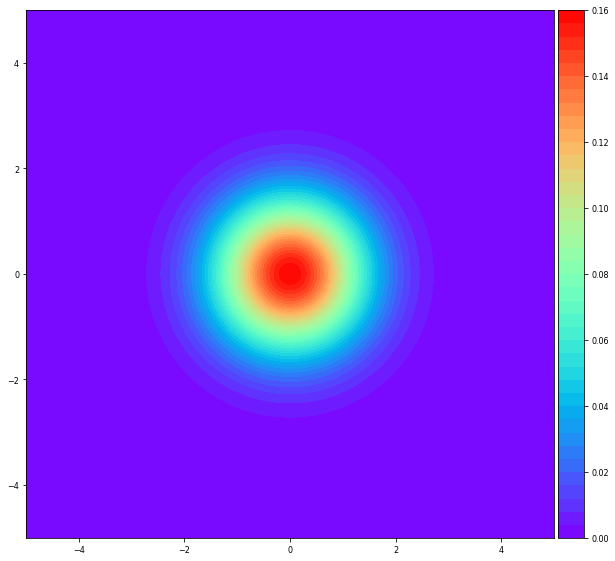
\includegraphics[width=0.49\linewidth]{figures/base_distribution.png}}
    \subfigure[]{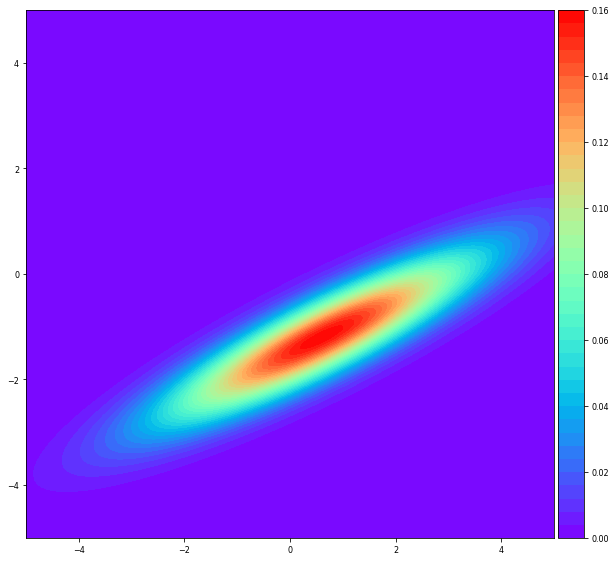
\includegraphics[width=0.49\linewidth]{figures/affine_transform.png}}
  \end{subfigmatrix}
    \caption{(a) Density of a Gaussian distribution with $\mu = [0, 0]$ and $\Sigma = I$
    (b) Density of the distribution that results from applying some affine transformation to
    the Gaussian distribution in (a)
    }
  \label{fig:affine}
\end{figure}

\subsubsection{PReLU Transformation}
Intuitively, introducing non-linearities endows normalizing flows with more flexibility to
represent complex distributions. This can be done in a similar fashion to the
activation functions used in neural networks. One example of that is the parameterized
rectified linear unit (PReLU) transformation. It is defined in the following manner, for
a $D$-dimensional input:
\begin{align}
f(\bm{z}) = [f_1(z_1), f_2(z_2), ..., f_D(z_D)],
\end{align} where
\begin{align}
f_i(z_i) =
    \begin{cases}
        z_i,              & \text{if } z_i\geq 0, \\
        \alpha z_i,       & \text{otherwise}.
    \end{cases}
\end{align}
In order for the transformation to be invertible, it is necessary
that $\alpha > 0$.
Let us define a function $j(.)$ as
\begin{align}
j(z_i) =
    \begin{cases}
       1 ,              & \text{if } z_i \geq 0, \\
       \alpha ,       & \text{otherwise};
    \end{cases}
\end{align}
it is trivial to see that the Jacobian of the transformation is a diagonal
matrix, whose diagonal elements are $j(z_i)$:
\begin{align}
  J(f(z)) =
  \begin{bmatrix}
      j(z_1) & & & \\
      & j(z_2) & & \\
      & & \ddots & \\
      & & & j(z_D)
  \end{bmatrix}.
\end{align}
With that in hand, it is easy to arrive at the log-absolute-determinant of this transformation's
Jacobian, which is given by $\sum_{i=1}^D \log \big| j(z_i) \big|$

\begin{figure}[!htb]
  \begin{subfigmatrix}{2}
    \subfigure[]{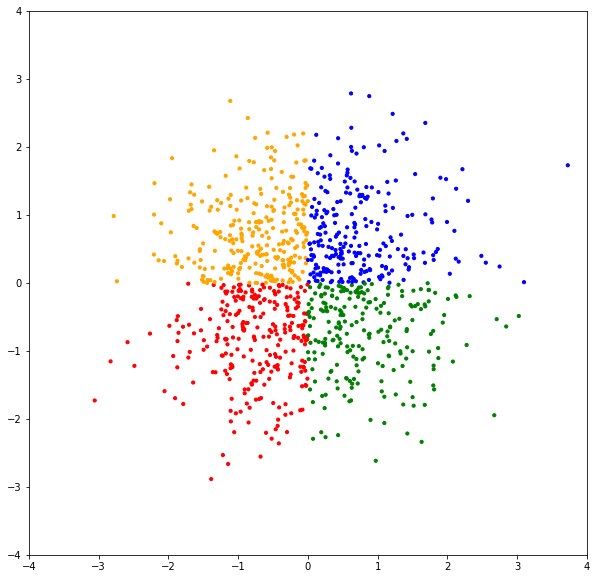
\includegraphics[width=0.49\linewidth]{figures/gaussian_in_quadrants.png}}
    \subfigure[]{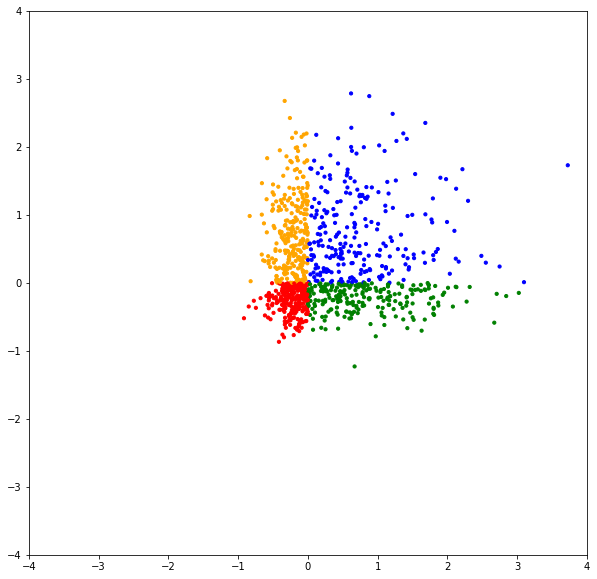
\includegraphics[width=0.49\linewidth]{figures/prelu_in_quadrants.png}}
  \end{subfigmatrix}
    \caption{(a) Samples from of a Gaussian distribution with $\mu = [0, 0]$ and $\Sigma = I$.
    The samples are colored according to the quadrant they belong to. (b) Samples from the
    distribuion in a) transformed by a PReLU transformation.}
  \label{fig:prelu}
\end{figure}

\begin{figure}[!htb]
  \begin{subfigmatrix}{3}
    \subfigure[]{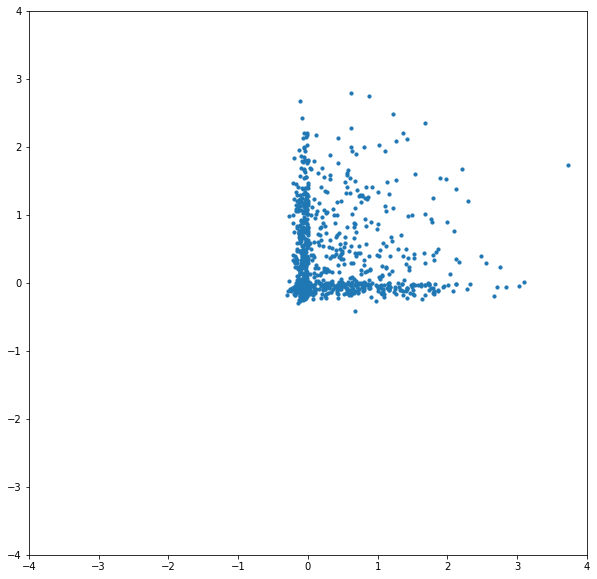
\includegraphics[width=0.31\linewidth]{figures/prelu_0_1.png}}
    \subfigure[]{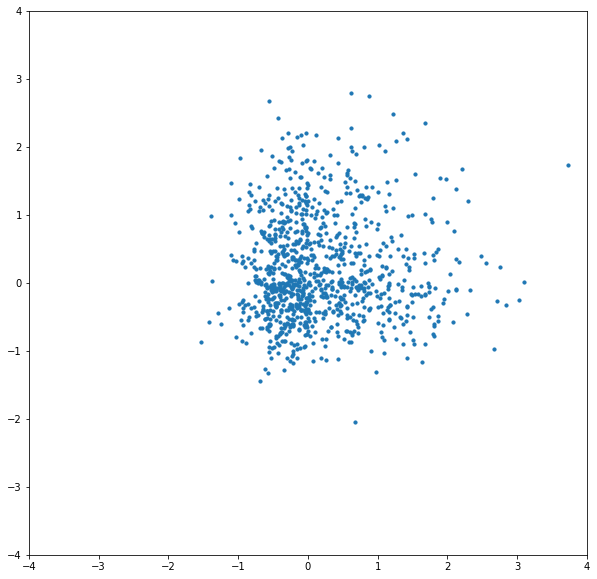
\includegraphics[width=0.31\linewidth]{figures/prelu_0_5.png}}
    \subfigure[]{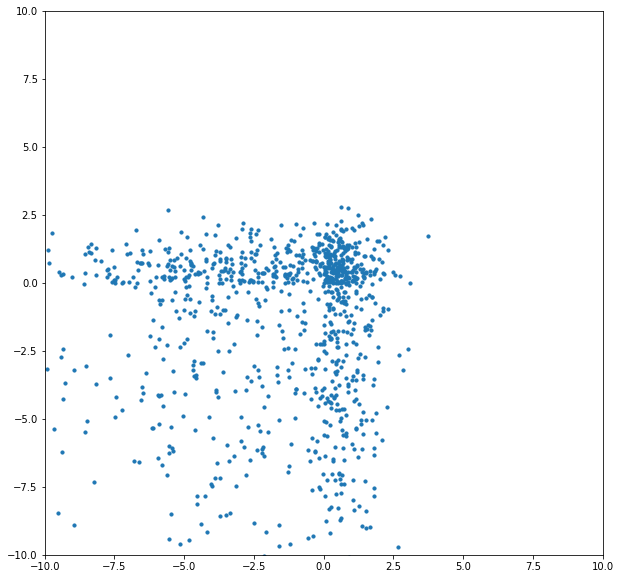
\includegraphics[width=0.31\linewidth]{figures/prelu_5.png}}
  \end{subfigmatrix}
    \caption{Samples from a Gaussian with $\mu = [0, 0]$ and $\Sigma = I$, transformed
    by PReLU transformations with different $\alpha$ parameters. (a) $\alpha = 0.1$
    (b) $\alpha = 0.5$ (c) $\alpha = 5$}
  \label{fig:prelu}
\end{figure}

\subsubsection{Batch-Normalization Transformation}
\textcite{real-nvp} propose a batch-normalization transformation, similar to
the well-known batch-normalization layer normally used in neural networks. This
transform simply applies a rescaling, given the batch mean $\tilde\mu$ and variance
${\tilde\sigma}^2$:
\begin{align}
    f(z) = \frac{z - \tilde\mu}{\sqrt{{\tilde\sigma}^2 + \epsilon}},
\end{align} where $\epsilon \ll 1$ is a term used to ensure that there never is
a division by zero. This transformation's Jacobian is trivial: 
\begin{align}
    \prod_{i=1}^D \frac{1}{\sqrt{{\tilde\sigma}_i^2 + \epsilon}}.
\end{align}

\subsubsection{Affine Coupling Transformation}
As mentioned previously, one of the active research challenges within the
normalizing flows framework is the search and design of transformations that
are sufficiently expressive and whose Jacobians are not computationally heavy. One brilliant
example of such transformations, proposed by \textcite{real-nvp}, is
called affine coupling layer.

This transformation is characterized by two arbitrary functions $s(.)$ and
$t(.)$, as well as a mask that splits an input $\bm{z}$ of dimension $D$ into
two parts, $\bm{z_1}$ and $\bm{z_2}$. In practice, $s(.)$ and $t(.)$ are neural
networks, whose parameters are to be optimized so as to make the transformation
approximate the desired output distribution. The outputs of $s(.)$ and $t(.)$
need to have the same dimension as $\bm{z_1}$. This should be taken into account when
designing the mask and the functions $s(.)$ and $t(.)$. The transformation is defined as:
\begin{align}
    \begin{cases}
    \bm{x_1} &= \bm{z_1} \odot \exp\big(s(\bm{z_2})\big) + t(\bm{z_2}) \\
    \bm{x_2} &= \bm{z_2}.
    \end{cases}
\end{align}
To see why this transformation is suitable to being used within the framework
of normalizing flows, let us derive its Jacobian.
\begin{itemize}
    \item $\frac{\partial \bm{x_2}}{\partial \bm{z_2}} = I$, because $\bm{x_2} = \bm{z_2}$.
    \item $\frac{\partial \bm{x_2}}{\partial \bm{z_1}}$ is a matrix of zeros, because $\bm{x_2}$ does not depend on $\bm{z_1}$.
    \item $\frac{\partial \bm{x_1}}{\partial \bm{z_1}}$ is a diagonal matrix,
        whose diagonal is simply given by $\exp\big(s(\bm{z_2})\big)$, since those values are
        constant w.r.t $\bm{z_1}$ and they are multiplying each element of $\bm{z_1}$.
    \item $\frac{\partial \bm{x_1}}{\partial \bm{z_2}}$ is not needed,
        as will become clear ahead.
\end{itemize}

Writing the above in matrix form:
%\[
%\begin{bmatrix}
%  \mbox{\huge$\frac{\partial \bm{x_1}}{\partial \bm{z_1}}$} & \mbox{\huge$\frac{\partial \bm{x_1}}{\partial \bm{z_2}}$} \\
%  \mbox{\huge$\frac{\partial \bm{x_2}}{\partial \bm{z_1}}$} & \mbox{\huge$\frac{\partial \bm{x_2}}{\partial \bm{z_2}}$} \\
%\end{bmatrix}
%\]


\begin{align}
    J_{f(z)} &=
        \begin{tikzpicture}[decoration=brace, baseline=-\the\dimexpr\fontdimen22\textfont2\relax ]
            \matrix (m) [matrix of math nodes,left delimiter=[,right delimiter={]}, ampersand replacement=\&] {
                \mbox{\Large$\frac{\partial \bm{x_1}}{\partial \bm{z_1}}$} \& \mbox{\Large$\frac{\partial \bm{x_1}}{\partial \bm{z_2}}$} \\
                \mbox{\Large$\frac{\partial \bm{x_2}}{\partial \bm{z_1}}$} \& \mbox{\Large$\frac{\partial \bm{x_2}}{\partial \bm{z_2}}$} \\
            };
%            \draw[decorate,transform canvas={xshift=-1.5em},thick] ($ (m-1-1.south west) +(0,3pt) $)
%                -- node[left=2pt] {$\frac{\partial \bm{x_1}}{\partial (.)}$} ($ (m-1-1.north west) -(0,3pt) $);
%            \draw[decorate,transform canvas={xshift=-1.5em},thick] ($ (m-2-1.south west) +(0,3pt) $)
%                -- node[left=2pt] {$\frac{\partial \bm{x_2}}{\partial (.)}$} ($ (m-2-1.north west) -(0,3pt) $);
%            \draw[decorate,transform canvas={yshift=0.5em},thick] ($ (m-1-1.north west) +(2pt,0) $)
%                -- node[above=2pt] {$\frac{\partial (.)}{\partial \bm{z_1}}$} ($ (m-1-1.north east) -(2pt,0) $);
%            \draw[decorate,transform canvas={yshift=0.5em},thick] ($ (m-1-2.north west) +(2pt,0) $)
%                -- node[above=2pt] {$\frac{\partial (.)}{\partial \bm{z_2}}$} ($ (m-1-2.north east) +(2pt,0) $);
        \end{tikzpicture} \\
    &=
        \begin{tikzpicture}[decoration=brace, baseline=-\the\dimexpr\fontdimen22\textfont2\relax ]
            \matrix (m) [matrix of math nodes,left delimiter=[,right delimiter={]}, ampersand replacement=\&] {
                \mbox{diag}\Big(\exp\big(s(\bm{z_2})\big)\Big) \& \mbox{\Large$\frac{\partial \bm{x_1}}{\partial \bm{z_2}}$} \\
                \mbox{\Large$\bm{0}$} \& \mbox{\Large$I$} \\
            };
        \end{tikzpicture}
\end{align} shows that the Jacobian matrix is (upper) triangular. Its determinant - the
only thing we need, in fact - is therefore easy to compute: it is simply the
product of the diagonal elements. Moreover, part of the diagonal is simply
composed of ones. The determinant, and the log-absolute-determinant become
\begin{align}
    \det\big(J_{f(z)}\big) &= \prod_i \exp\big(s(\bm{z_2}^{(i)})\big) \\
    \log \Big|\det\big(J_{f(z)}\big)\Big| &= \sum_i s(\bm{z_2}^{(i)}),
\end{align} where $\bm{z_2^{(i)}}$ is the $i$-th element of $\bm{z_2}$.
Since a single affine coupling layer does not transform all of the elements in
$\bm{z}$, in practice several layers are composed, and each layer's mask is changed
so as to make all dimensions affect each other. This can be done, for instance, with
a checkerboard pattern, which alternates for each layer. In the case of image inputs,
the masks can operate at the channel level.

\subsubsection{Masked Autoregressive Flows}
Another ingenious architecture for normalizing flows has been proposed by \textcite{maf}.
It is called masked autoregressive flow (MAF). Let $\bm{z}$ be a sample from
some base distribution, with dimension $D$. MAF transforms $\bm{z}$ into an
observation $\bm{x}$, of the same dimension, in the following manner:
\begin{align}
x_i = z_i \exp(\alpha_i) + \mu_i \\
(\mu_i, \alpha_i) = g(\bm{x_{1:i-1}}).
\end{align}
In the above expression $g$ is some arbitrary function. The inverse transform of
MAF is trivial, because, like the affine coupling layer, MAF uses $g$ to parameterize
a shift, $\mu$, and a log-scale, $\alpha$, which translates to the fact that the
function $g$ itself does not need to be inverted:
\begin{align}
z_i = (x_i - \mu_i)\exp(-\alpha_i).
\end{align}
Moreover, the autoregressive structure of the transformation constrains the
Jacobian to be triangular, which renders the determinant effortless to compute: 
\begin{align}
\det\big( J_{f(\bm{z})} \big) &= \prod_{i=1}^{D} \exp(\alpha_i), \\
\log \Big| \det \big( J_{f(\bm{z})} \big) \Big| &= \sum_{i=1}^{D} \alpha_i.
\end{align}
As stated above, the function $g$ used to obtain $\mu_i$ and $\alpha_i$ can be
arbitrary. However, in the original paper, the function proposed a masked
autoencoder for distribution estimation (MADE), as described by \textcite{MADE}.

Much like the partitioning in the affine coupling layer, the assumption of
autoregressiveness (and the ordering of the elements of $\bm{x}$
for which that assumption is held) carries an inductive bias with it. Again,
like with the affine coupling layer, this effect is minimized in practice by
stacking layers with different element orderings.

\subsection{Fitting Normalizing Flows}

Generally speaking, normalizing flows can be used in one of two scenarios:
(direct) density estimation, where the goal is to optimize the parameters
so as to make the model approximate the distribution of some observed set of data;
in a variational inference scenario, as way of having a flexible variational
posterior. The second scenario is out of the scope of this work.

The task of density estimation with normalizing flows reduces to finding the
optimal parameters of a parametric model. In general, there are two ways to go about estimating
the parameters of a parametric model,
given data: MLE and MAP. In the case of normalizing flows, MLE is the usual
approach\footnote{In theory it is possible to place a prior on the normalizing
flow's parameters and do MAP estimation. To accomplish this, similar strategies
to those used in Bayesian Neural Networks would have to be used.}. To fit a normalizing
flow via MLE, a gradient based optimizer is used to minimize
$\hat{\mathcal{L}}(\bm\theta) = - \mathbb{E}[\log p(\bm{x}|\bm\theta)]$.
However, this expectation is generally not accesible, since we have only
finite samples of $\bm{x}$. Because of that, the parameters are estimated
by optimizing an approximation of that expectation: $ - \frac{1}{N} \sum_{i=1}^N \log p(\bm{x_i} | \bm\theta)$.

To perform optimization on this objective, stochastic gradient descent (SGD) - and
its variants -  is the most commonly used algorithm. In general terms, SGD is an
approximation of gradient descent, which rather than using the actual gradient,
at time step $t$, to update the variables under optimization, works by computing
several estimates of that gradient and using those estimates instead. This is
done by partitioning the data in mini-batches, and computing the loss function
and respective gradients over those mini-batches. This way, one pass through
data - an \emph{epoch} - results in several parameter updates.

\chapter{Variational Mixture of Normalizing Flows}
\label{chapter:vmonf}

\section{Introduction}
\label{section:vmonf-intro}

As mentioned in sections \ref{section:probmodellatvar} and \ref{section:mmodels},
the ability of leveraging domain knowledge to endow a probabilistic model with
structure is often useful. The goal of this work is to devise a model that combines
the flexibility of Normalizing Flows with the ability to exploit class-membership
structure. Specifically, such model would be able to learn $K$ Normalizing Flows,
each responsible for one of $K$ clusters in a dataset.

\section{Model Definition}

Let us define a Mixture Model as in \ref{section:mmodels}, where each of the $K$
components is a Normalizing Flow. For simplicity, consider that all of the $K$
Normalizing Flows have the same architecture \footnote{This is not a requirement,
and in cases where we have classes with different levels of complexity, we can
have components with different architectures. However, the training procedure
does not guarantee that that the most flexible Normalizing Flow is "allocated"
to the most complex cluster. This is definitely an interesting direction for future
research.}, i.e., they are all composed of the same stack of transformations,
but they each have their own parameters.

Additionally, let $q(z|\bm{x};\gamma)$ be a neural network with a softmax output, with
parameters $\bm\gamma$. This network will receive as input an instance from the
data, and produce the probability of that instance belonging to each of the
$K$ classes.

Recall the Evidence Lower Bound given in \ref{eq:elbokldiv}\footnote{Here the
dependence of $q$ on $x$ is made explicit}:
\begin{equation*}
    \text{ELBO} = \mathbb{E}_q [\log p(\bm{x}, z)] - \mathbb{E}_q [\log q(z|\bm{x})]
\end{equation*}

Let us rearrange it:
\begin{align}
    \text{ELBO} &= \mathbb{E}_q [\log p(\bm{x}|z)] + \mathbb{E}_q [\log p(z)] - \mathbb{E}_q [\log q(z|\bm{x})]
        \label{eq:threepartelbo} \\
    \text{ELBO} &= \mathbb{E}_q [\log p(\bm{x}|z) + \log p(z) - \log q(z|\bm{x})] \label{eq:simplerelbo}
\end{align}

Since $q(z|\bm{x})$ is given by the forward-pass of a neural network, and is therefore
straightforward to obtain, the expectation in \ref{eq:simplerelbo} is given by
computing the expression inside the expectation for each possible value of $z$,
and summing the obtained values, weighed by the probabilities given by the variational posterior.
Thus, the whole ELBO is easy to compute, provided that each of the terms inside
the expectation is itself easy to compute. Let us consider each of those terms:
\begin{itemize}
    \item $\log p(\bm{x}|z)$ is the log-likelihood of $\bm{x}$ under the Normalizing
        Flow indexed by $z$. It was shown in the previous chapter how to compute
        this.
    \item $\log p(z)$ is the log-prior of the component weights. For simplicity,
        let us assume this is set by the modeller. When nothing is known about
        the component weights, the best assumption is that they are uniform.
        Nevertheless, as will be shown empirically, this too can be optimized.
    \item $- \log q(z|\bm{x})$ is the negative logarithm of the output of the encoder.
\end{itemize}

For a better intuition about each of these terms, it is useful to review the last
paragraph of the first subsection of section \ref{subsubsection:kldiv}.

I call this model Variational Mixture of Normalizing Flows (VMoNF). For an overview of
the model, consider figures \ref{fig:plate} and \ref{fig:modeloverview}

\begin{figure}[!htb]
  \centering
  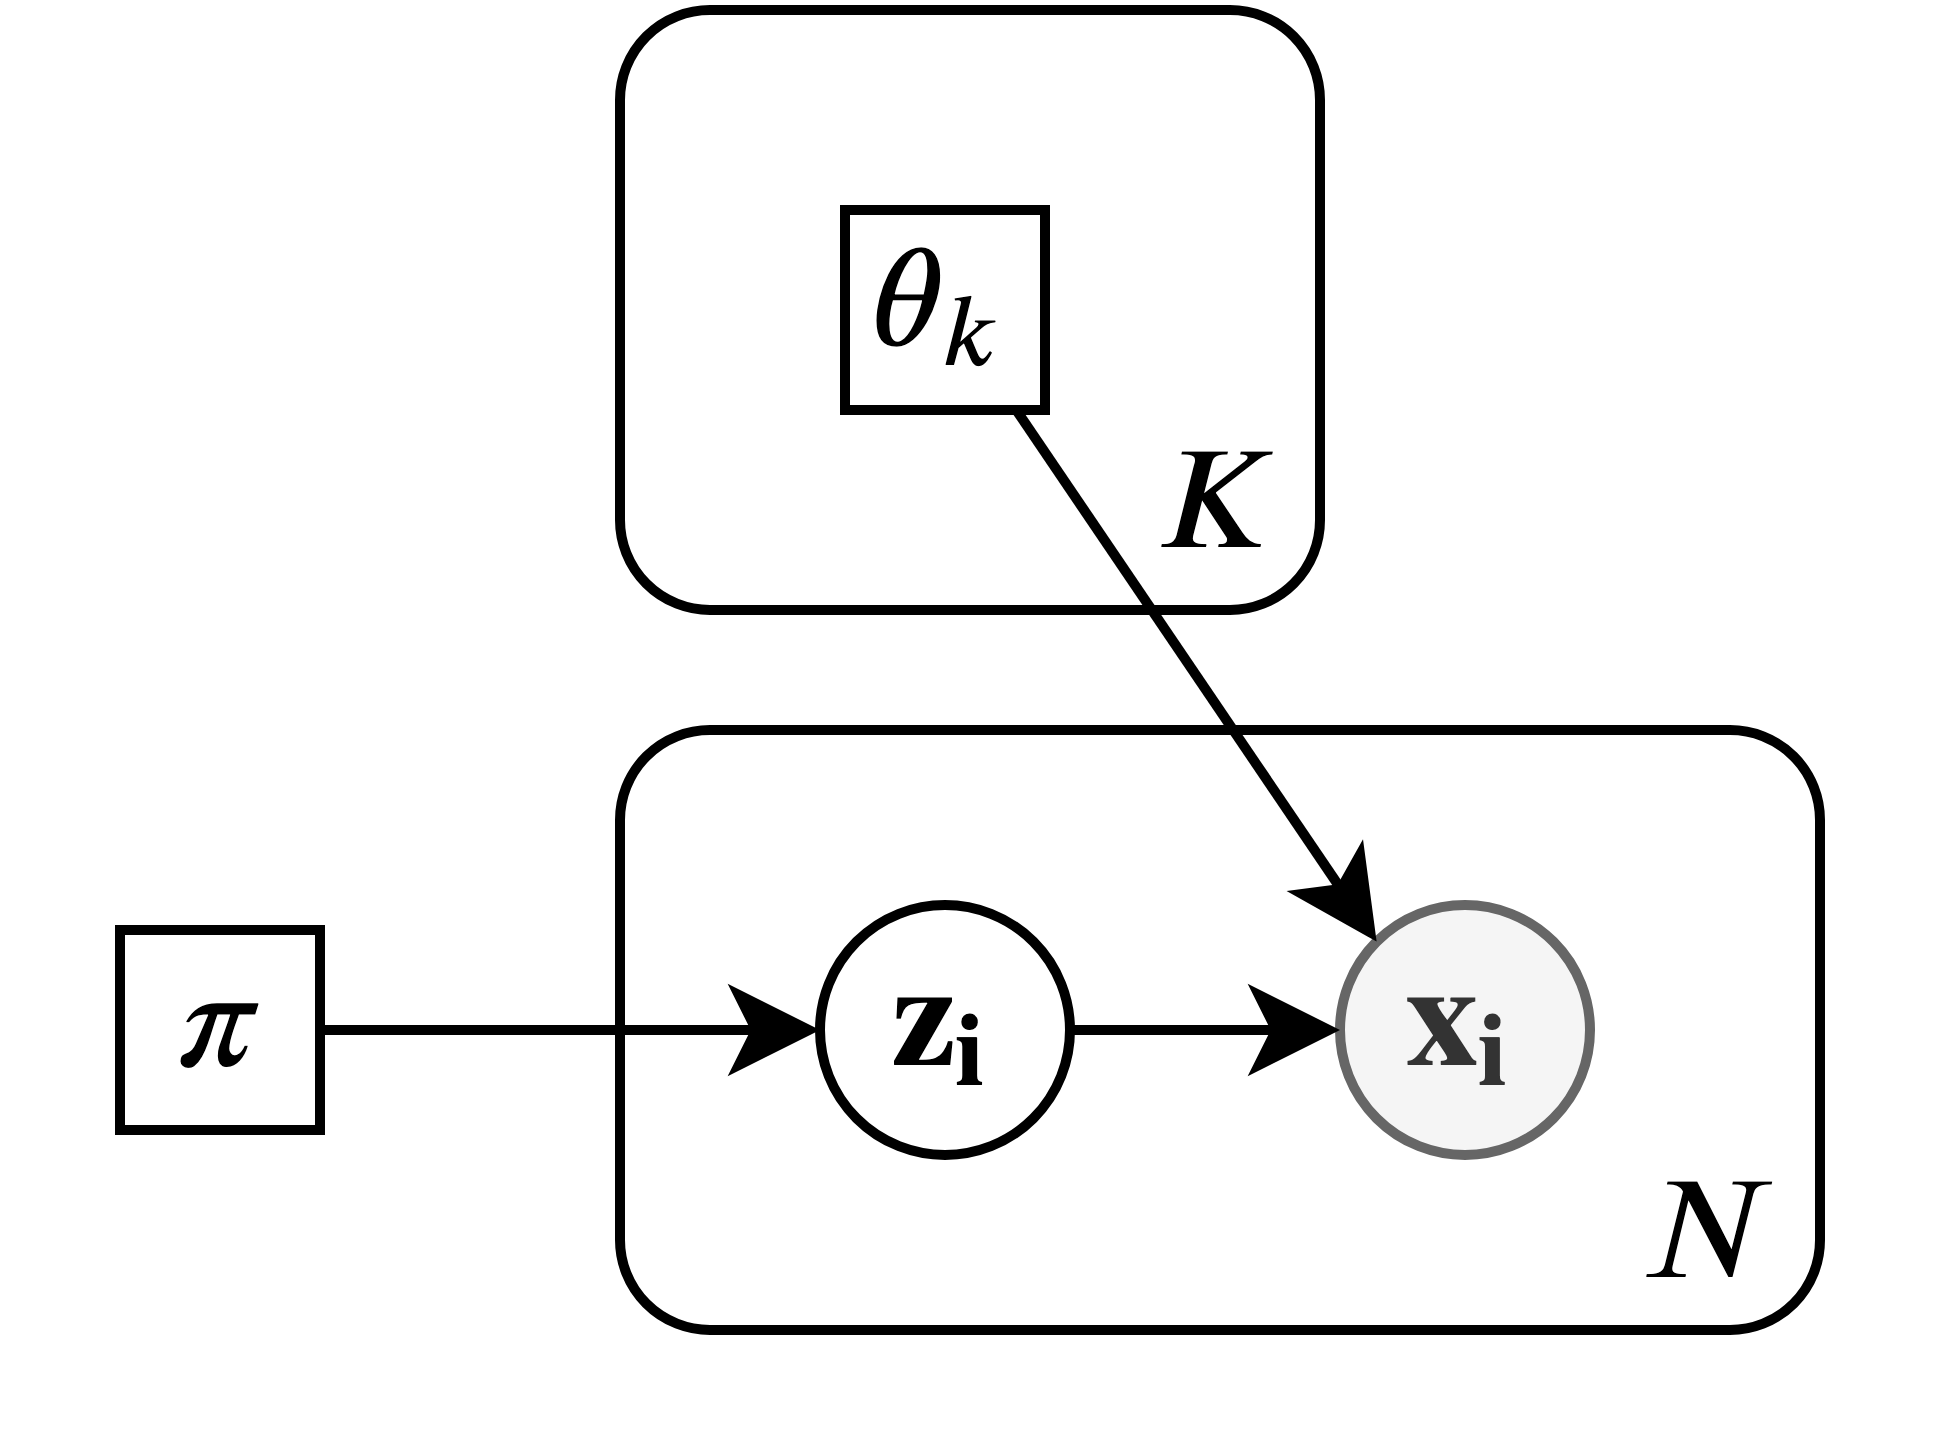
\includegraphics[width=0.5\linewidth]{figures/plate_diagram.png}
  \caption{Plate diagram of a Mixture of $K$ Normalizing Flows. $\bm\theta_k$ is the
    parameter vector of component $k$.}
  \label{fig:plate}
\end{figure}

\begin{figure}[!htb]
  \centering
  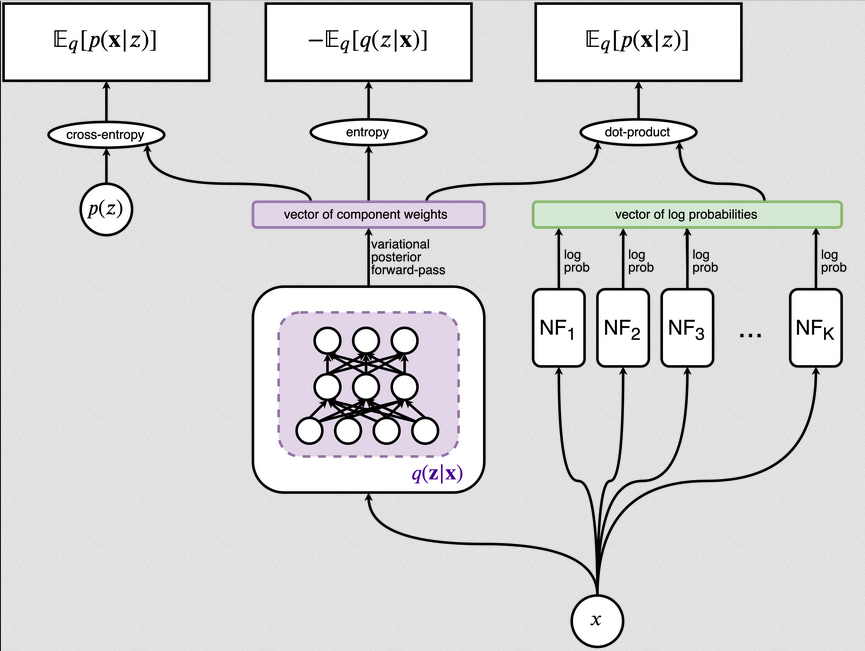
\includegraphics[width=0.85\linewidth]{figures/train_overview.png}
  \caption{Overview of the training procedure.}
  \label{fig:modeloverview}
\end{figure}

In a similar fashion to how the Variational Auto-Encoder, proposed in \cite{vaepaper}
works, a VMoNF is fitted by jointly optimizing the parameters of the variational
posterior $q(z|\bm{x}; \bm\gamma)$ and the parameters of the generative process
$p(\bm{x}|z; \bm\theta)$.

\chapter{Experiments}
\label{chapter:experiments}

In this chapter, the proposed model is applied to two synthetic datasets (Pinwheel
and Two-circles) and one real-world dataset (MNIST). On one of the synthetic
datasets, one shortcoming of the model is brought to attention, but is overcome
in a semi-supervised setting. On the real-world dataset, the model's clustering
capabilities are evaluted, as well as its capacity to model complex distributions.

All experiments were conducted using RealNVP (the model proposed in \autocite{real-nvp})
as the normalizing flow model for the mixture components. Moreover, a technique
inspired in \autocite{mixae} was employed to improve training speed and quality
of results. This consisted of dividing the inputs of the softmax layer in
the variational posterior by a temperature value, $t$, which was made to follow
an exponential decay schedule during training. Intuitively, this makes the
variational posterior \q{more certain} as training moves on, while allowing all
components to be generally exposed to the whole data, in the initial epochs.
This incentivizes components to not be \q{subtrained} in the initial epochs and
then prematurely discarded by the variational posterior.

\section{Toy datasets}
\subsection{Pinwheel dataset}

This dataset is constituted by five non-linear \q{wings}. See figure \ref{fig:pinwheel}
for the results of running the model on this dataset. As expected, the variational
posterior has learned to partition the space so as to attribute each \q{wing} to
a component of the mixture. This partitioning is imperfect in regions of space
that have low probability for every component.

\begin{figure}[!htb]
  \begin{subfigmatrix}{2}
    \subfigure[]{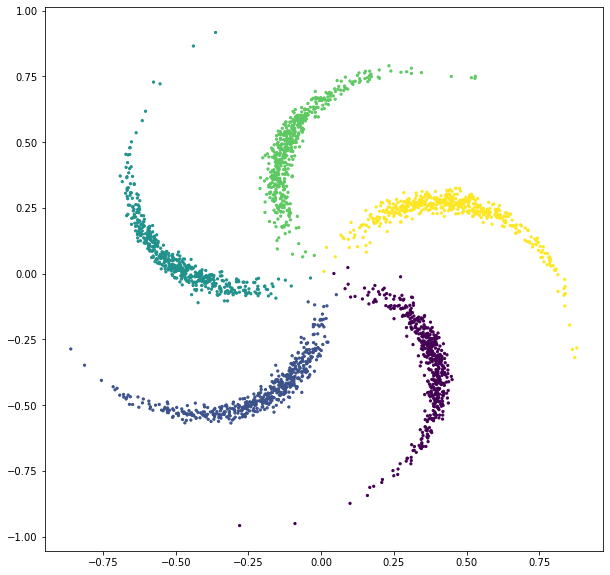
\includegraphics[width=0.49\linewidth]{figures/original_pinwheel.png}}
    \subfigure[]{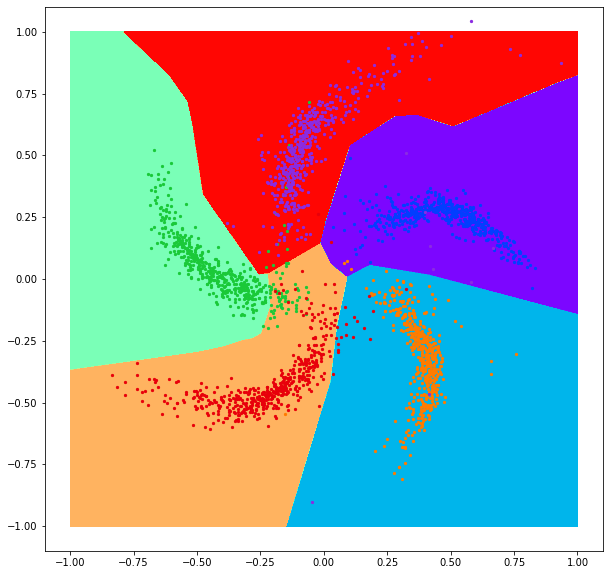
\includegraphics[width=0.49\linewidth]{figures/trained_pinwheel.png}}
  \end{subfigmatrix}
    \caption{(a) Original dataset. (b) Samples from the learned model. Each
dot is colored according to the component it was sampled from. The background
colors denote the regions where each component has maximum probability assigned
by the variational posterior. (Note that the background colors were chosen
so as to not match the dot colors, otherwise it dots wouldn't be visible)}
  \label{fig:pinwheel}
\end{figure}

This experiment consisted of training on 2560 data points, 512 per class; using
the Adam (\autocite{adam}) optimizer, with a learning rate of 0.001, with a
mini-batch size of 512, during 400 epochs. The variational posterior was parameterized
by a multi-layer perceptron, with 1 hidden layer of dimension 3, and with a
softmax output. Each component of the mixture was a RealNVP with 8 blocks, each
block with multi-layer perceptrons, with 1 hidden layer of dimension 8, as the
$s(.)$ and $t(.)$ functions of the affine coupling layers.

\subsection{Two-circles dataset}
This dataset consists of two concentric circles. The experiment on this dataset,
visible on figure \ref{figure:twocircles}, makes evident one shortcoming of this
model: the way in which the variational posterior partitions space is
not necessarily guided by the intrisic structure in the data. In the case of
the two-circles dataset, it was found that the most common space partitioning
induced by the model consisted simply of splitting space in half. However, in
a semi-supervised setting, this behaviour can be corrected and the model
successfully learns to separate the two circles, as is visible in figure
\ref{fig:twocircles-semisup}. In this setting, the model was pretrained on
the labeled instances for some epochs and then trained with the normal procedure.
In the semi-supervised setting the model has the chance to refine both the
variational posterior and each of the components, thus making better use of
the unlabeled data in the unsupervised phase of the training. As is clearly
visible in figure \ref{fig:twocircles-semisup}, the model struggles with
learning full, closed, circles. This is because it is unable to \q{pierce a hole}
in the base distribution, due to the nature of the transformations that are
applicable. Thus, to model a circle, the model has to learn to stretch the blob
formed by the base distribution, and \q{bend it over itself}. This difficulty
is also what keeps the model from learning a structurally interesting solution
in the fully unsupervised case: it is easier to learn to distort space so as to
learn a multimodal distribution that models half of the two circles.

The unsupervised learning experiment consisted of training on 1024 datapoints,
512 per class; using the Adam (\autocite{adam}) optimizer, with a learning rate
of 0.001, with a mini-batch size of 128, during 500 epochs.
The semi-supervised learning experiment consisted of training on 1024 unlabeled
datapoints, 512 per class; and 32 labeled data points, 16 per class. The model
was first pretrained during 300 epochs solely on the 32 labeled data points, using
the labels to selectively optimize each component of the mixture, as well as
to optimize the variational posterior by minimizing a binary cross-entropy loss.
After pretraining, the model was trained by interweaving supervised epochs - like
in pretraining - with unsupervised epochs. Optimization was carried out using the
Adam (\autocite{adam}) optimizer, with a learning rate of 0.001, with a mini-batch size
of 128, during 500 epochs.
For both the unsupervised and the semi-supervised experiments, the neural network
used to parameterize the variational posterior was a multi-layer perceptron, with
2 hidden layers of dimension 16, and with a softmax output. Each component of the
mixture was a RealNVP with 10 blocks, each block with multi-layer perceptrons,
with 1 hidden layer of dimension 8, as the $s(.)$ and $t(.)$ functions of the
affine coupling layers.

\begin{figure}[!htb]
  \begin{subfigmatrix}{2}
    \subfigure[]{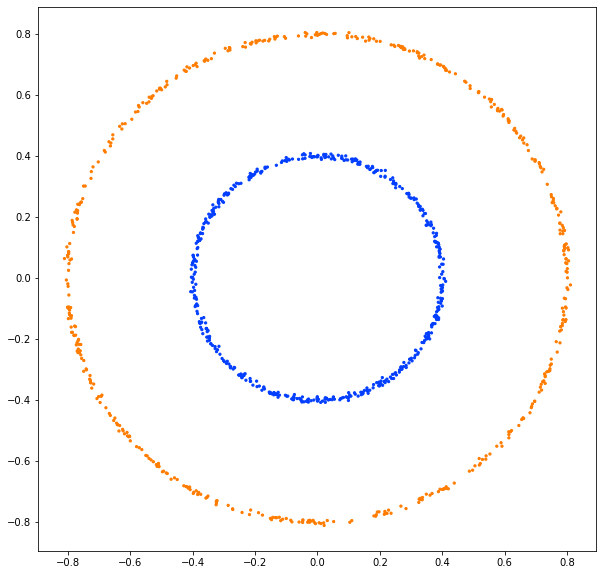
\includegraphics[width=0.49\linewidth]{figures/original_2_circles.png}}
    \subfigure[]{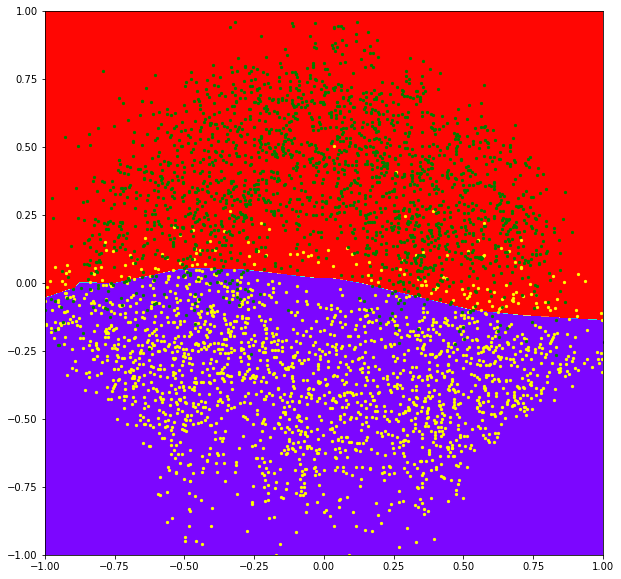
\includegraphics[width=0.49\linewidth]{figures/trained_2_circles.png}}
  \end{subfigmatrix}
    \caption{(a) Original dataset. (b) Samples from the learned model, without
    any labels. Coloring logic is the same as in \ref{fig:pinwheel}. (c) Samples
    from semi-supervised scenario.}
\label{fig:twocircles}
\end{figure}

\begin{figure}[!htb]
  \begin{subfigmatrix}{2}
    \subfigure[]{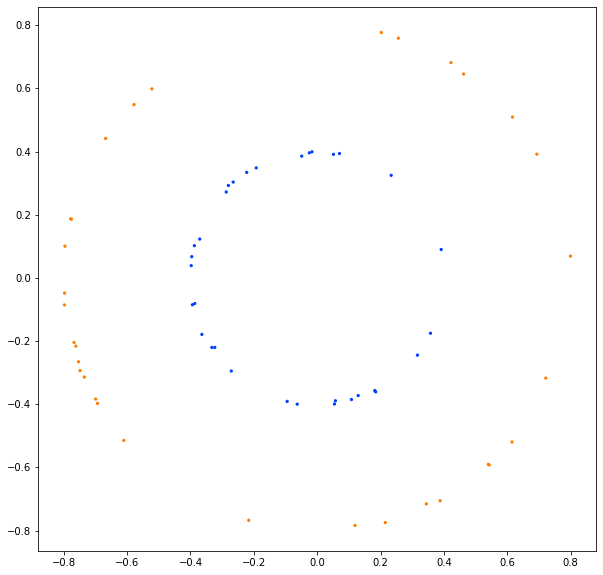
\includegraphics[width=0.49\linewidth]{figures/labeled_2_circles.png}}
    \subfigure[]{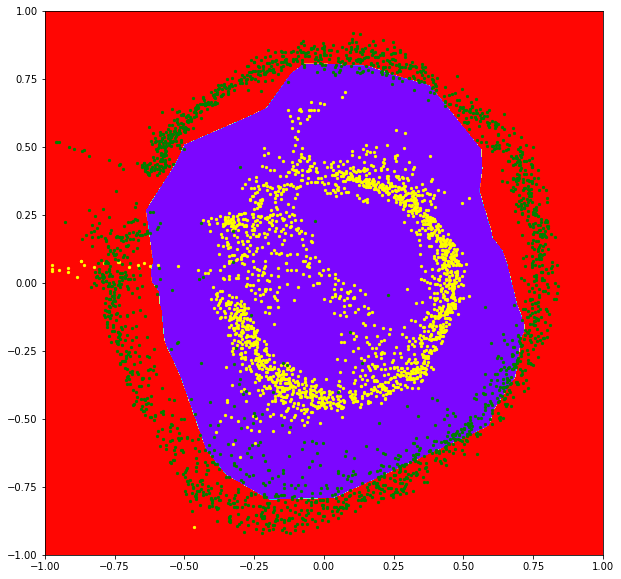
\includegraphics[width=0.49\linewidth]{figures/trained_2_circles_semisup.png}}
  \end{subfigmatrix}
    \caption{(a) Labeled points used in semi-supervised scenario. (b) Samples
    from the model trained in the semi-supervised scenario.}
\label{fig:twocircles-semisup}
\end{figure}

\section{Real-world dataset}
In this section, the proposed model is evaluated in the well-known MNIST
dataset(\autocite{MNIST}). This dataset consists of pixel-matrices of images of
handwritten digits. The grids are of dimension 28 x 28, and were flattened
to vectors of dimension 784 for training. For this experiment, only the images
corresponding to the digits from 0 to 4 were considered. The normalizing
flow model used for the components was a MAF, with 5 blocks, whose internal MADE
layers had 1 hidden layer of dimension 200. The variational posterior was parameterized
by a multi-layer perceptron, with 1 hidden layer of dimension 512. The model
was trained for 100 epochs, with a mini-batch size of 100. The Adam optimizer
was used, with a learning rate of 0.0001, and with a weight decay parameter of
0.000001. In figure \ref{mnist_samples}, samples from the components obtained
after training can be seen. Moreover, a normalized contingency table is presented,
where the performance of the variational posterior as a clustering function
can be assessed. Note that the cluster indices induced by the model have no
semantic meaning.

\begin{figure}[!htb]
  \centering
  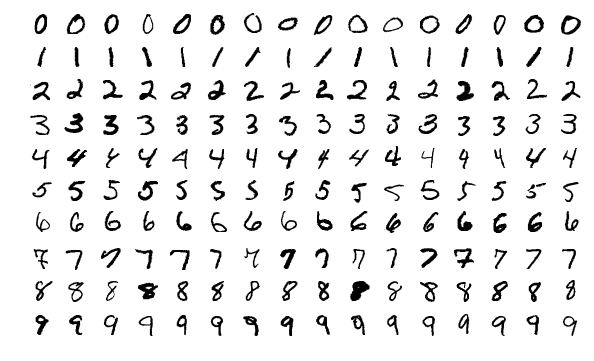
\includegraphics[width=0.85\linewidth]{figures/trained_mnist.png}
  \caption{Samples from the fitted mixture components. Each row is sampled
  from the same component}
  \label{fig:mnist_samples}
\end{figure}

\begin{table}[h]
\centering
\begin{tabular}{lrrrrr}
\toprule
 cluster index&         0 &         1 &         2 &         3 &         4 \\
true label &           &           &           &           &           \\
\midrule
0    &  0.028702 &  0.002533 &  0.947662 &  0.019754 &  0.001351 \\
1    &  0.000000 &  0.015426 &  0.001187 &  0.003263 &  0.980125 \\
2    &  0.019470 &  0.854481 &  0.045821 &  0.019637 &  0.060591 \\
3    &  0.001631 &  0.114011 &  0.046648 &  0.820910 &  0.016800 \\
4    &  0.000685 &  0.005649 &  0.648237 &  0.000856 &  0.344574 \\
\bottomrule
\end{tabular}
\caption{Normalized contingency table for the clustering induced by the model}
\label{table:contingency}
\end{table}

From table \ref{table:contingency} and figure \ref{fig:mnist_samples} it's possible
to see that although there is some confusion, the model successfully clusters
the MNIST digits.

\chapter{Conclusions}
\label{chapter:conclusions}

Insert your chapter material here...


% ----------------------------------------------------------------------
\section{Achievements}
\label{section:achievements}

The major achievements of the present work...


% ----------------------------------------------------------------------
\section{Future Work}
\label{section:future}

A few ideas for future work...



%\begin{figure}[!t]
%\centering
%\includegraphics[width=2.5in]{myfigure}
% where an .eps filename suffix will be assumed under latex, 
% and a .pdf suffix will be assumed for pdflatex; or what has been declared
% via \DeclareGraphicsExtensions.
%\caption{Simulation results for the network.}
%\label{fig_sim}
%\end{figure}

%\begin{figure*}[!t]
%\centering
%\subfloat[Case I]{\includegraphics[width=2.5in]{box}%
%\label{fig_first_case}}
%\hfil
%\subfloat[Case II]{\includegraphics[width=2.5in]{box}%
%\label{fig_second_case}}
%\caption{Simulation results for the network.}
%\label{fig_sim}
%\end{figure*}
%

% can use a bibliography generated by BibTeX as a .bbl file
% BibTeX documentation can be easily obtained at:
% http://mirror.ctan.org/biblio/bibtex/contrib/doc/
% The IEEEtran BibTeX style support page is at:
% http://www.michaelshell.org/tex/ieeetran/bibtex/
%\bibliographystyle{IEEEtran}
% argument is your BibTeX string definitions and bibliography database(s)
%\bibliography{IEEEabrv,../bib/paper}
%
% <OR> manually copy in the resultant .bbl file
% set second argument of \begin to the number of references
% (used to reserve space for the reference number labels box)

\printbibliography

\end{document}

